\documentclass[12pt, a4paper]{report}
\usepackage{graphicx, array, amsthm, amssymb, amsmath, algorithm, algpseudocode, float, xcolor, thmtools, thmbox}
\usepackage[english]{babel}

\makeatletter
\renewcommand\thmbox@headstyle[2]{\bfseries #1}
\makeatother
\newtheorem[style=M,bodystyle=\normalfont]{theorem}{Theorem}
\newtheorem[style=M,bodystyle=\normalfont]{corollary}{Corollary}
\newtheorem[style=M,bodystyle=\normalfont]{lemma}{Lemma}
\newtheorem[style=M,bodystyle=\normalfont]{definition}{Definition}


\title{Image Analysis And Computer Vision\\ \textit{Theory}}
\author{Christian Rossi}
\date{Academic Year 2023-2024}

\begin{document}

\maketitle

\newpage

\begin{abstract}
    The topics of the course are: 
    \begin{itemize}
        \item Introduction.
        \item Camera sensors: transduction, optics, geometry, distortion
        \item Basics on Projective geometry: modelling basic primitives (points, lines, planes, conic sections, quadric surfaces) and projective spatial transformations and  projections.
        \item Camera geometry, and single view analysis: calibration, image rectification, localization of 3D models.
        \item Multi-view analysis: 3D shape reconstruction, self-calibration, 3D scene understanding.
        \item Linear filters and convolutions, space-invariant filters, Fourier Transform, sampling and aliasing. 
        \item Nonlinear filters: image morphology and morphology operators (dilate, erode, open, close), median filters.
        \item Edge detection and feature detection techniques. feature matching and feature tracking along image sequences.
        \item Inferring parametric models from noisy data (including outliers), contour segmentation, clustering, Hough Transform, Ransac (random sample consensus). 
        \item Applications: object tracking, object recognition, classification.
    \end{itemize}
\end{abstract}

\newpage

\tableofcontents

\newpage

\chapter{Optical Sensors}
    \section{Photocamera}
    \begin{definition}
    The \emph{photocamera} is an optical sensor; this means that produces data using electric transducers. It uses an optical system that select the direction of the incoming light at each 
    element of its screen made with millions of photosensitive elements. Most of the actual cameras can capture up to 30-60 frames per second. 
    \end{definition}
    For simplicity, we suppose that the optical system of a photocamera is a single lens that is:
    \begin{itemize}
        \item Spherical: the lens is obtained by intersecating two spheres. 
        \item Thin: the distance between the center of the two spheres is almost identical to the sum of the diameter of them. 
    \end{itemize}
    This simplifies the computation of the path of the ray crossing the lens. In fact, the refraction of the light when crossing a border between two media is given by the Snell's law: 
    \[\dfrac{\sin{\theta_2}}{\sin{\theta_1}}=\dfrac{n_1}{n_2}\]
    where: 
    \begin{itemize}
        \item $\theta_1$ and $\theta_2$ are the angles between the normal at the surface and the direction of the light ray. 
        \item $n_1$ and $n_2$ are the refraction indexes of the two materials.
    \end{itemize}
    \begin{figure}[H]
        \centering
        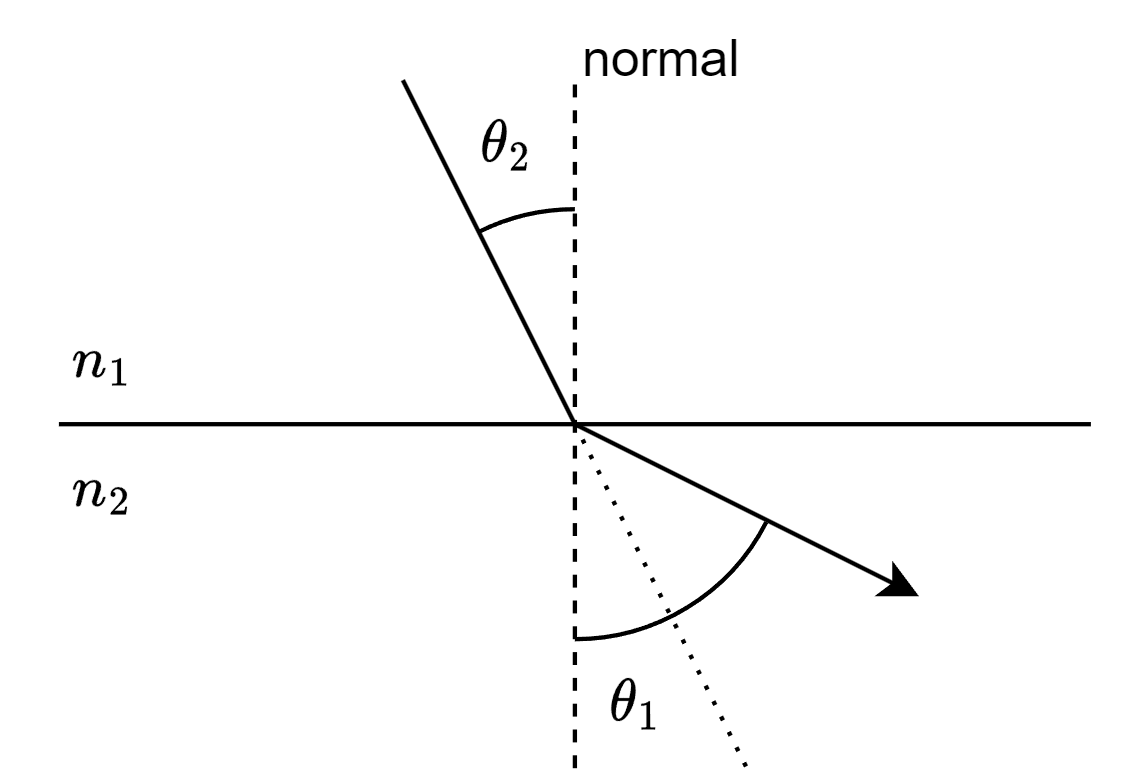
\includegraphics[width=0.5\linewidth]{images/refraction.png}
        \caption{Snell's law}
    \end{figure}
    Other than that, we also have to hypothesize that the light forms small inclination angles with the optical axis.
    \begin{definition}
        The \emph{optical axis} is the straight line that connects the centre of the two spheres that are used to form the lens. 
    \end{definition}
    The angles of a ray passing trough the centres of the spheres can be calculated as follows: 
    \[\alpha_1=\dfrac{y_1}{\rho_1} \:\:\:\:\:\: \alpha_2=-\dfrac{y_2}{\rho_2}\]
    \begin{figure}[H]
        \centering
        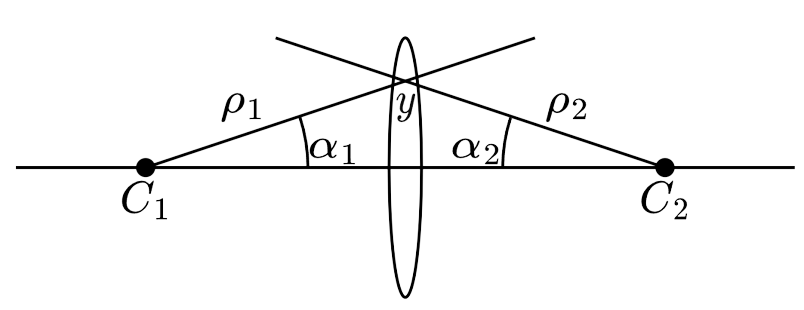
\includegraphics[width=0.5\linewidth]{images/y.png}
    \end{figure}
    Since we have a simplified lens, it is possible to say that:
    \[y_1=y_2=y\]
    
    \section{Deviation of a light ray crossing a thin lens}
    \begin{figure}[H]
        \centering
       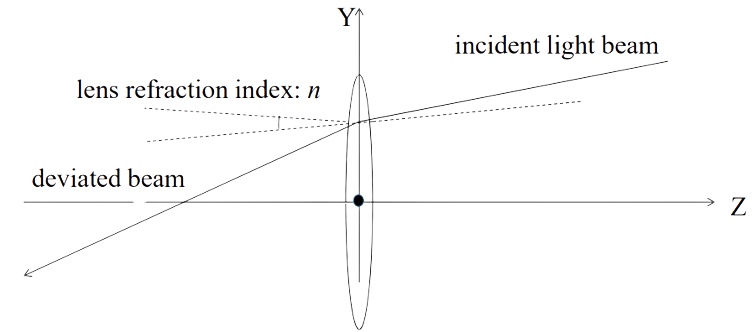
\includegraphics[width=0.5\linewidth]{images/ray.png}
   \end{figure}
    Given a lens with refraction $n$ we have that the following equeations are valid:
    \[\dfrac{\theta-\alpha_1}{\theta^{'}-\alpha_1} \Rightarrow \dfrac{\sin{(\theta-\alpha_1)}}{\sin{(\theta^{'}-\alpha_1)}}=n\]
    \[\dfrac{\theta^{''}-\alpha_2}{\theta^{'}-\alpha_2} \Rightarrow \dfrac{\sin{(\theta^{''}-\alpha_2)}}{\sin{(\theta^{'}-\alpha_2)}}=n\]
    where:
    \begin{itemize}
        \item $\theta$ is the incident angle (light on the lens). 
        \item $\theta^{'}$ is the angle in the lens (not visible in the image). 
        \item $\theta^{''}$ is the angle after the lens.
    \end{itemize}
    Comparing the two equations it is possible to find the difference between the input angle $\theta$ and the output angle $\theta^{''}$ that is: 
    \[\delta \theta=y(n-1)\left( \dfrac{1}{\rho_1} + \dfrac{1}{\rho_2}\right)\]
    It is possible to see that the first term $(n-1)$ is due to the matter of the lens and the second $\left( \frac{1}{\rho_1} + \frac{1}{\rho_2}\right)$ depend on the curvature 
    of the surface. 

    \section{Focalization of parallel light rays}
    \begin{figure}[H]
        \centering
       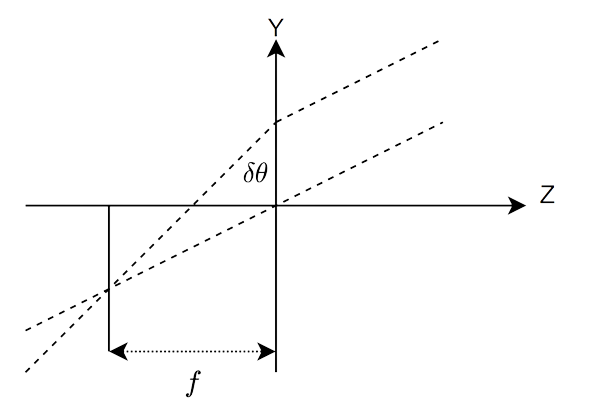
\includegraphics[width=0.5\linewidth]{images/focalization.png}
    \end{figure}
    In the image we have one ray that passes trough the centre of the lens and the other that passes in another point but it is parallel to the first one. So we have that: 
    \begin{itemize}
        \item $Y=0$, so we have that the deviation of the ray is null and proceed without being deviated. 
        \item $Y=f \cdot \delta \theta \Rightarrow f=\dfrac{1}{(n-1)\left( \dfrac{1}{\rho_1} + \dfrac{1}{\rho_2}\right)}$. 
    \end{itemize}
    This means that all the rays that proceed in parallel meets in one common point on the focal point $Z$, with a distance from the $Y$ axis equal to: 
    \[Z=-f\]


\end{document}